\section{Тёмное вещество. Ключевые наблюдательные свидетельства.}
\begin{figure}[H]
    \centering
    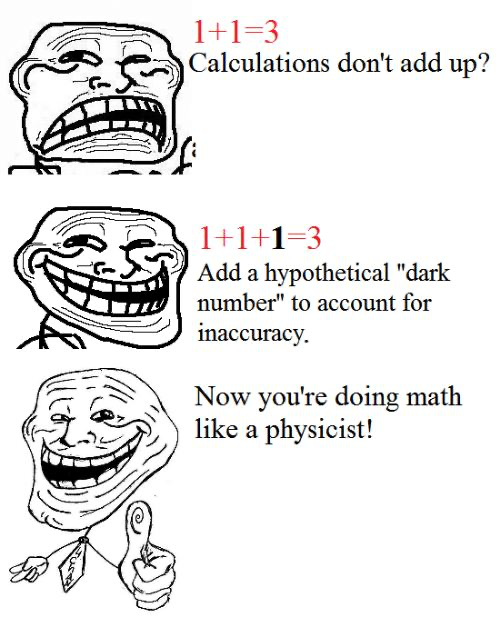
\includegraphics[scale=0.5]{17_memes.png}
    \caption{Билет вкратце.}
    \label{fig:memes}
\end{figure}
\subsection{Тёмное вещество}
Тёмная материя в астрономии и космологии, а также в теоретической физике — гипотетическая форма материи, не участвующая в электромагнитном взаимодействии и поэтому недоступная прямому наблюдению. Составляет порядка четверти массы-энергии Вселенной и проявляется только в гравитационном взаимодействии. Понятие тёмной материи введено для теоретического объяснения проблемы скрытой массы в эффектах аномально высокой скорости вращения внешних областей галактик и гравитационного линзирования (в них задействовано вещество, масса которого намного превышает массу обычной видимой материи); среди прочих предложенных оно наиболее удовлетворительно.
\subsection{Ключевые наблюдательные свидетельства.}
\subsubsection{Вращение звёзд в галактиках.}
\begin{figure}[H]
    \centering
    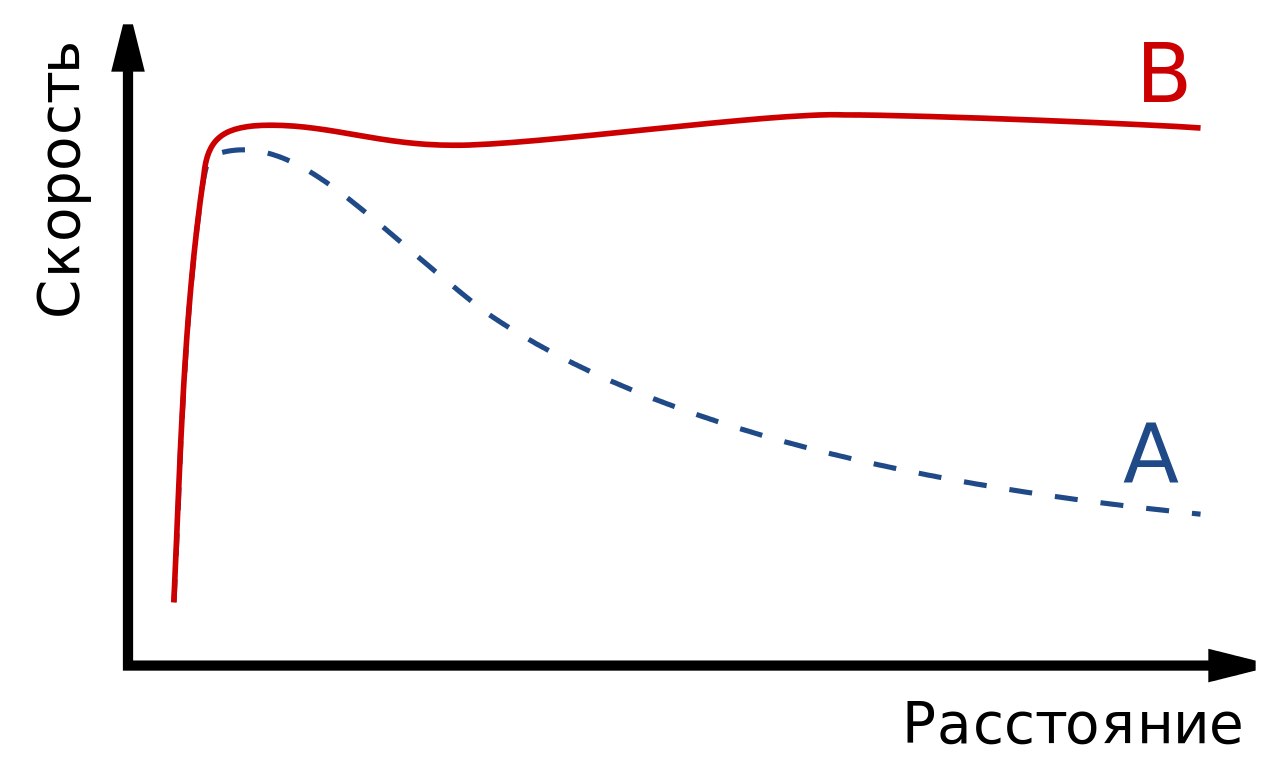
\includegraphics[scale=0.2]{17_curve.png}
    \caption{Кривая вращения галактики: (A) ожидаемая; (B) реальная.}
    \label{fig:galaxy_curve}
\end{figure}
Кривые вращения галактик, демонстрирующие отсутствие убывания скорости вращения на периферии звёздных дисков. Наиболее простым объяснением этого эффекта является наличие у галактик массивных невидимых гало, дающих большой вклад в их массы.
\subsubsection{Движение галактик-спутников и шаровых скоплений возле массивных галактик.}
Мелкие галактики-спутники движутся вокруг крупных, подчиняясь тем же законам, что и звёзды на периферии обычных галактик, таким образом являясь пробными телами такого же рода, но на большем масштабе, что позволяет делать выводы о распределении гравитационного потенциала таких массивных галактик. Анализ данных для нашей и других галактик подтвердил, что общая масса каждой галактики в несколько раз превышает суммарную массу её звёзд.
\subsubsection{Большие системы}
Динамика систем галактик от двойных галактик до галактических скоплений. Анализ лучевых скоростей их членов даёт характерный разброс скоростей галактик, что позволяет оценить полные массы этих систем. Таким образом выявлено, что тёмная материя присутствует на всех уровнях галактической иерархии, причём её доля растёт с увеличением масштаба: в двойных системах она превышает вклад видимой материи в несколько раз, а в скоплениях галактик (состоящих из сотен и тысяч объектов) — в десятки или сотни раз.
\subsubsection{Распределение горячего газа в эллиптических галактиках}
Рентгеновское излучение горячего газа в гигантских эллиптических галактиках и их скоплениях, зарегистрированное такими орбитальными обсерваториями как «Эйнштейн», «ROSAT», «XMM-Newton» и «Чандра». С помощью рентгеновских телескопов определяется распределение поверхностной яркости (в рентгеновском диапазоне) и температуры таких объектов в двумерной проекции, на основании этих характеристик строится радиальное распределение плотности и температуры газа, что даёт возможность получить массовый профиль галактики или скопления, исходя из условия гидростатического равновесия. Это важное преимущество такого метода, поскольку иные дают лишь значение полной массы объекта. Масса одних лишь звёзд и газа, согласно расчётам, недостаточна для удержания входящего в галактики и скопления горячего газа, если не учесть тёмную материю. Такой горячий газ составляет лишь порядка 15 \% всей массы скоплений, светящаяся видимая материя — ещё меньше, всего 5 \%, и оставшиеся 80 \% представляют собой тёмную материю. При этом радиальное распределение газа (в зависимости от расстояния до центра объекта) примерно повторяет гипотетическое распределение тёмной материи — профиль Наварро — Френка — Уайта.
\subsubsection{Гравитационное линзирование}
Гравитационное линзирование — отклонение света удалённых объектов гравитационным полем находящихся на его пути массивных скоплений, ввиду чего изображения более удалённых галактик, проецирующихся на некое наблюдаемое скопление, оказываются искажёнными (слабое гравитационное линзирование) или даже расщепляются на несколько «копий» (сильное гравитационное линзирование). По характеру этих искажений становится возможным восстановить распределение и величину массы внутри скопления, в том числе скрытой.
